\documentclass[11pt]{article}

\usepackage[margin=1in]{geometry}
\usepackage[T1]{fontenc}
\usepackage[utf8]{inputenc}
\usepackage{lmodern}
\usepackage{microtype}
\usepackage{amsmath, amssymb}
\usepackage{booktabs}
\usepackage{xcolor}
\usepackage{hyperref}
\usepackage{enumitem}
\usepackage{longtable}
\usepackage{graphicx}
\usepackage{float}

\hypersetup{
  colorlinks=true,
  linkcolor=blue!50!black,
  urlcolor=blue!50!black,
  citecolor=blue!50!black
}

\title{Async Chunking for Delayed VLA Control:\\Toy Benchmark Note and Next Steps}
\author{Working Note for \texttt{async\_chunking\_compare}}
\date{April 19, 2026}

\begin{document}
\maketitle

\begin{abstract}
This note summarizes a lightweight point-mass experiment for comparing delayed chunked-control strategies inspired by recent VLA deployment ideas. The current artifact is useful for intuition, but it is not yet a finished benchmark. The main value of the toy is to separate several physical intuitions: synchronous replanning wastes wall-clock time, naive asynchronous replanning suffers stale-state misalignment, train-time prefix conditioning can partially internalize delay-awareness, and future-state alignment can improve handoff quality when the planner reasons about the execution-time state rather than the stale one.
\end{abstract}

\section{Executive Summary}

The current implementation compares six methods:
\begin{enumerate}[leftmargin=1.5em]
  \item \texttt{Synchronous}: wait for the next chunk before continuing.
  \item \texttt{Naive Async}: overlap planning and execution, but plan from stale state.
  \item \texttt{RTC Hard Stitch}: a deliberately crude negative control that freezes the committed prefix without actual inpainting guidance.
  \item \texttt{Train-Time Prefix}: a toy learned continuation model that predicts a constant postfix action from stale state plus committed prefix.
  \item \texttt{History + Prefix}: the same idea plus a short recent-action history window, as a proxy for a recurrent or history-aware controller.
  \item \texttt{VLASH}: roll the committed prefix forward and plan from the estimated future execution state.
  \item \texttt{VLASH + Reflex}: VLASH plus a small per-step residual controller.
\end{enumerate}

The main result is narrow but useful:
\begin{itemize}[leftmargin=1.5em]
  \item In the static-goal setting, \texttt{VLASH} is the strongest method on settle time and final error.
  \item The toy \texttt{Train-Time Prefix} baseline closes part of the gap without explicit future rollout, but it is slower and less reliable than \texttt{VLASH}.
  \item The new \texttt{History + Prefix} baseline does not close the gap further in this toy, which is itself useful evidence that short action history is not enough here.
  \item \texttt{RTC Hard Stitch} fails badly, but that should be read only as evidence that hard prefix freezing is insufficient. It is not a faithful RTC baseline.
  \item In the moving-goal setting, the ranking is mixed. \texttt{VLASH} remains competitive, but the current metrics do not show clean dominance over all baselines.
\end{itemize}

\section{Experimental Setup}

The simulator is a one-dimensional point mass with position \(x\), velocity \(v\), control step \(\Delta t = 0.02\) s, chunk horizon \(H = 18\), and inference delay \(d = 8\) by default. The environment injects Gaussian velocity disturbances with standard deviation \(0.035\) per step.

Two scenarios are currently reported:
\begin{itemize}[leftmargin=1.5em]
  \item \textbf{Static goal:} fixed target at \(x = 10.0\).
  \item \textbf{Moving goal:} sinusoidal target motion with amplitude \(1.2\) and period \(2.6\) s.
\end{itemize}

The static-goal evaluation emphasizes settling and endpoint accuracy. The moving-goal evaluation emphasizes tracking quality, specifically the fraction of time inside the tolerance band and the tail mean absolute tracking error. The latest script also exports per-trial CSVs for uncertainty-aware analysis and adds standard-error bars to the aggregate plots.

\paragraph{Important limitation.}
This is structurally close to an oracle-versus-student comparison. \texttt{VLASH} uses an exact rollout of the same nominal dynamics used by the environment, and both \texttt{Train-Time Prefix} and \texttt{History + Prefix} are trained on labels derived from the same analytic planner. That makes the current result much narrower than a full method benchmark.

\section{Static-Goal Results}

\begin{figure}[H]
  \centering
  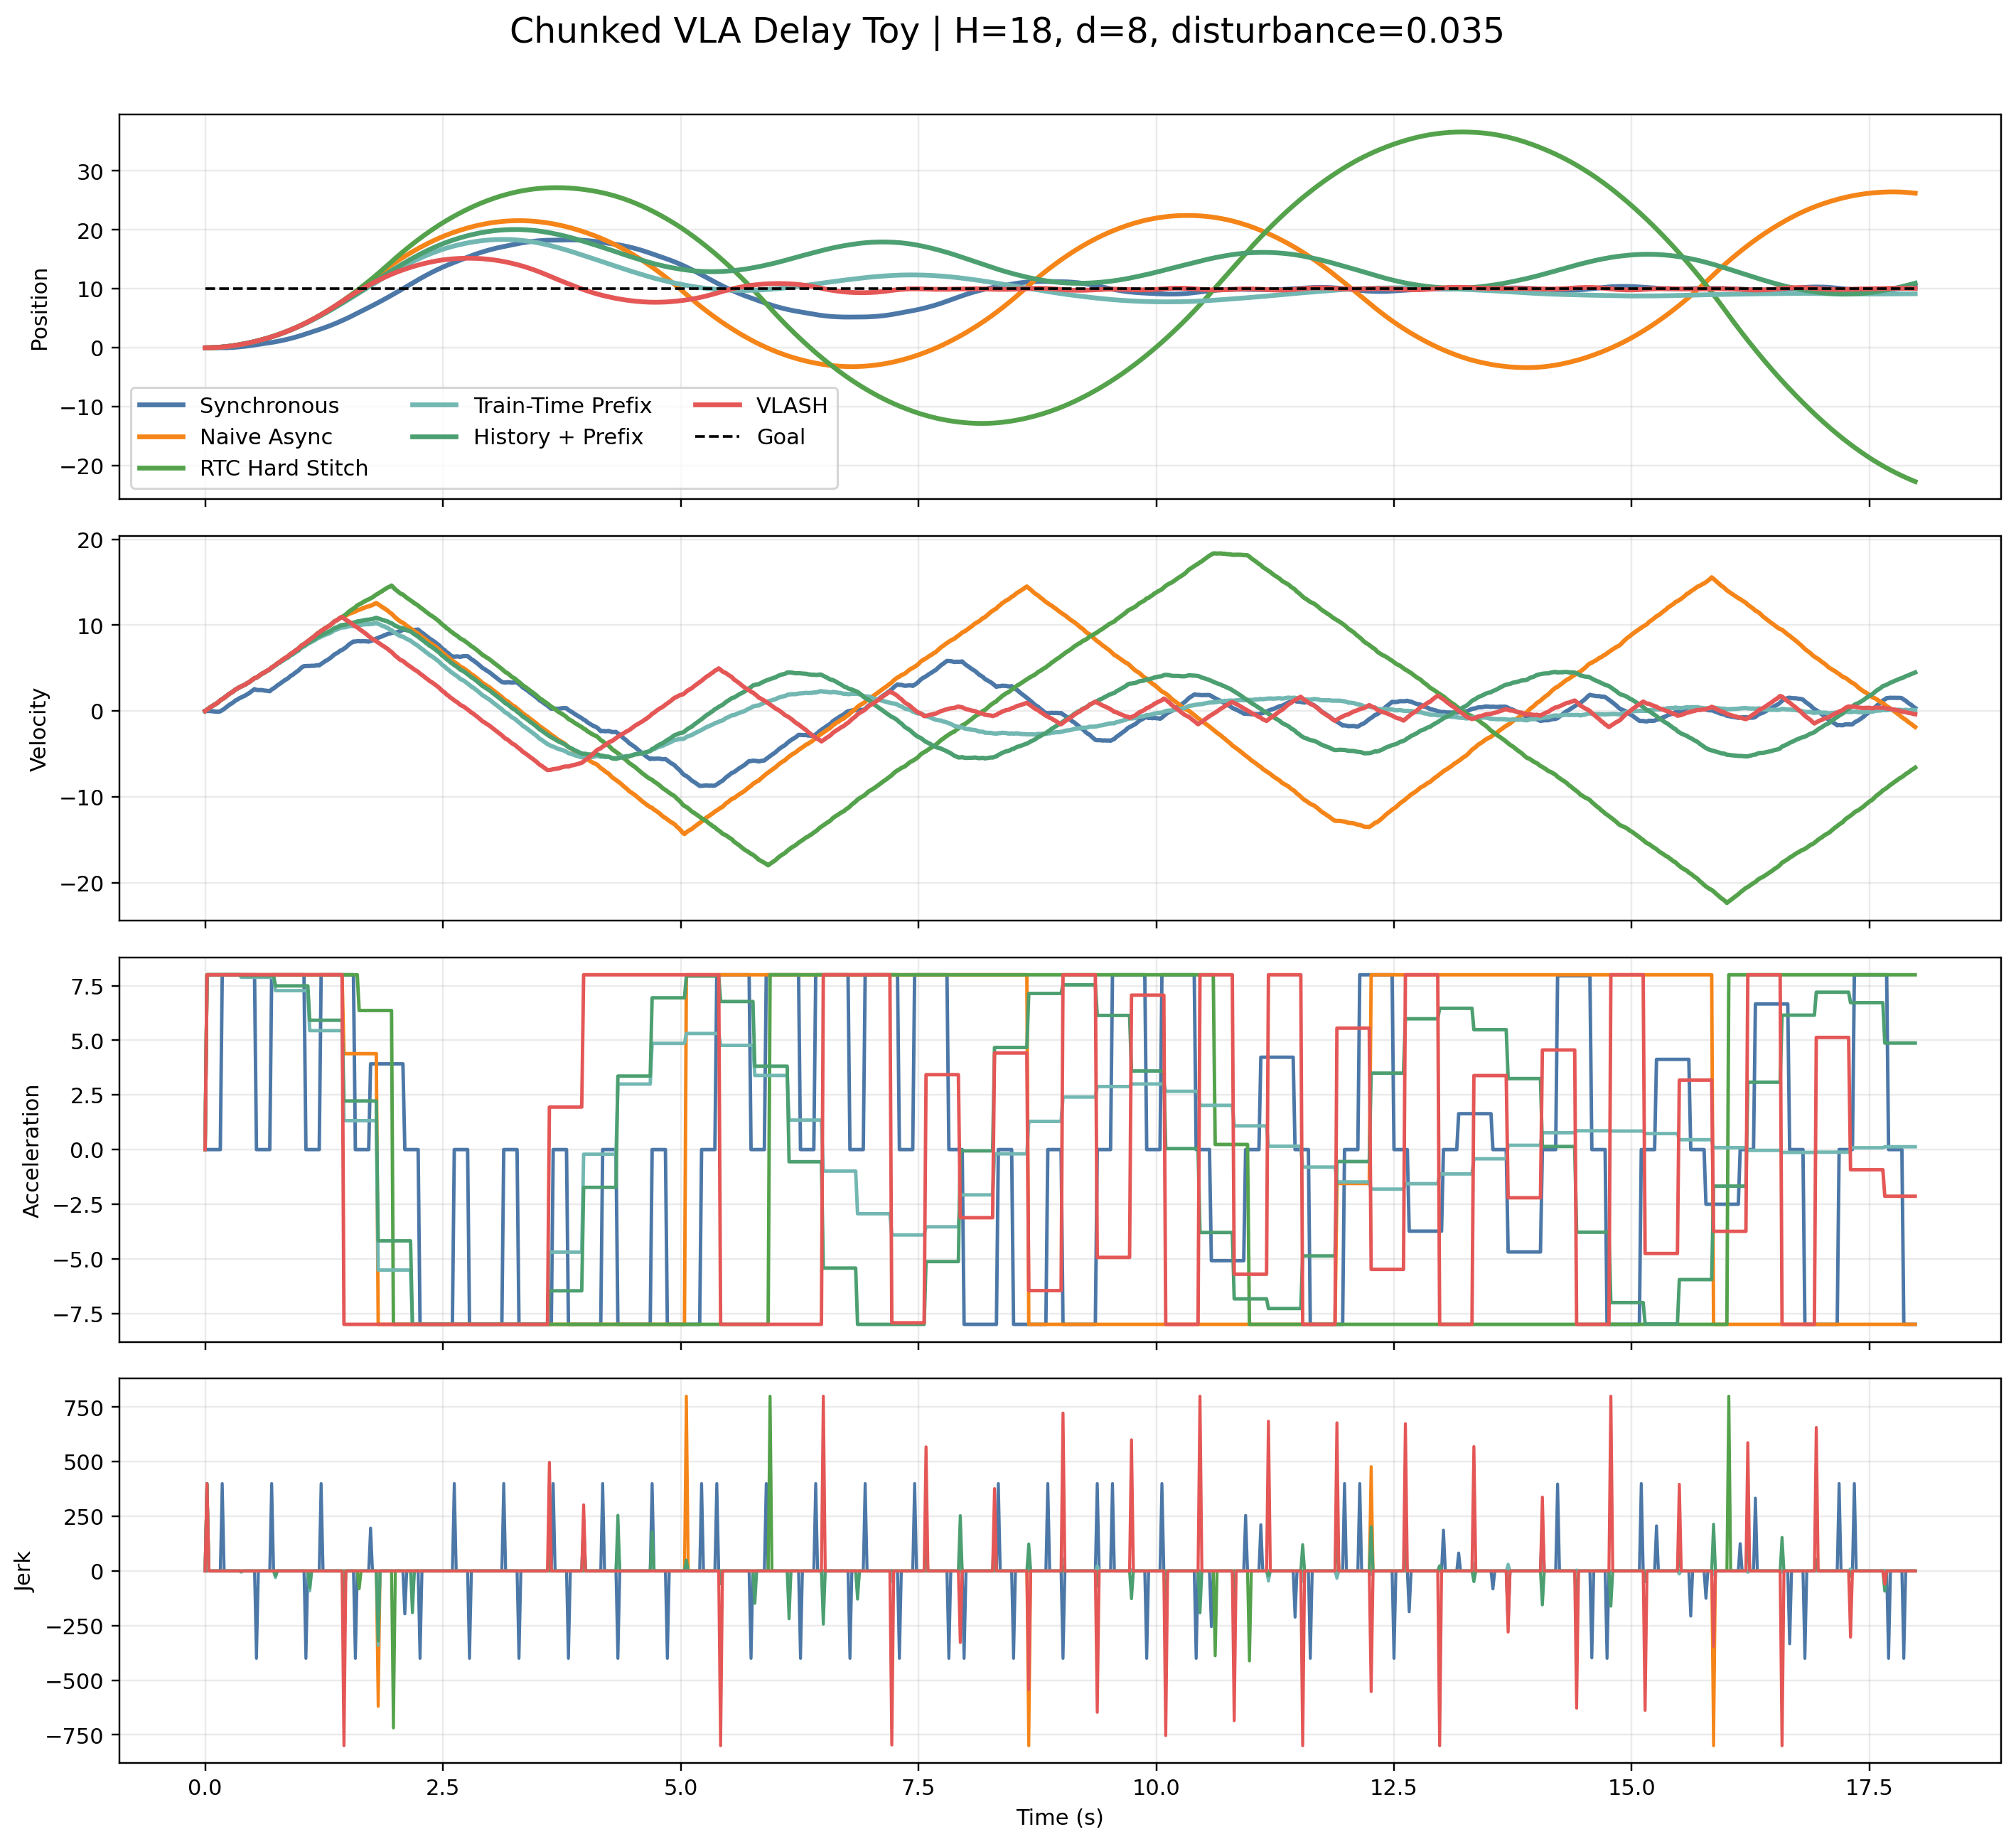
\includegraphics[width=\textwidth]{../outputs/async_chunking_static_single_run.png}
  \caption{Single-run static-goal comparison. The main qualitative pattern is visible: synchronous replanning is stable but slow, naive async oscillates, hard stitching diverges, train-time prefix conditioning dampens the stale-state pathology, and VLASH reaches the target fastest.}
\end{figure}

\begin{figure}[H]
  \centering
  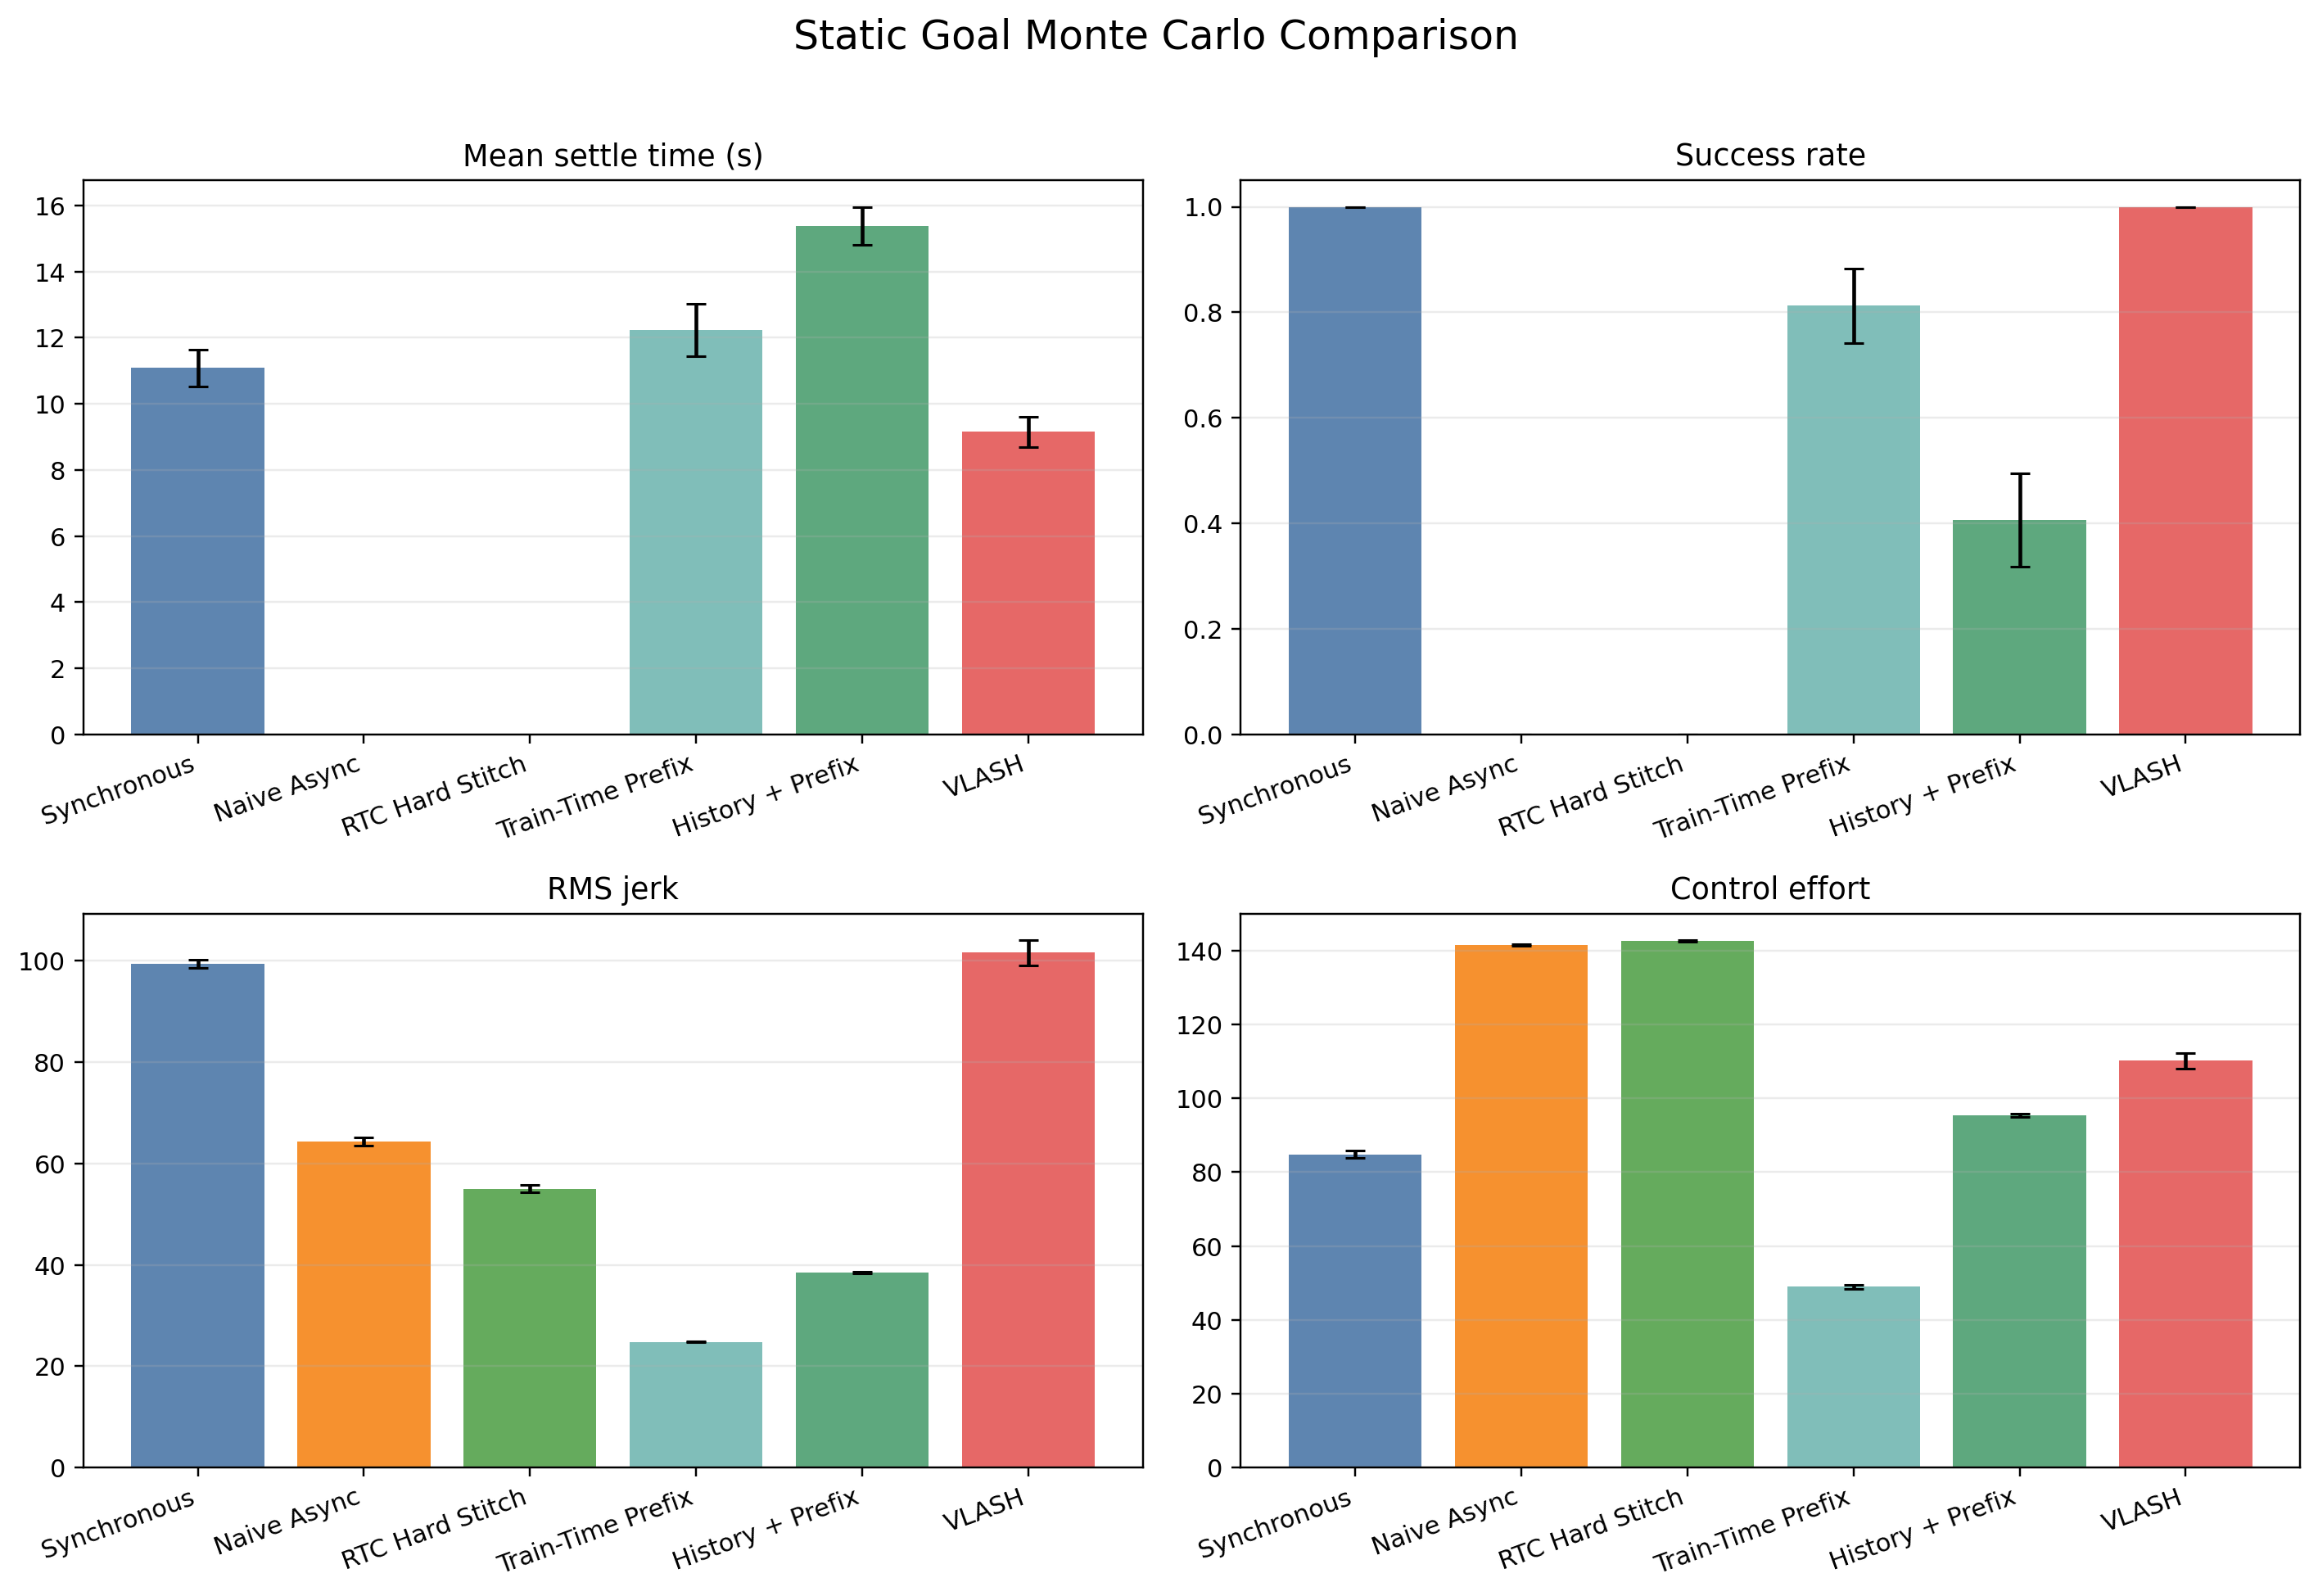
\includegraphics[width=\textwidth]{../outputs/async_chunking_static_monte_carlo.png}
  \caption{Monte Carlo aggregates for the static-goal setting.}
\end{figure}

\begin{table}[H]
\centering
\begin{tabular}{lrrrr}
\toprule
Method & Success (\%) & Mean settle (s) & Final error & RMS jerk \\
\midrule
Synchronous & 100.0 & 11.09 & 0.164 & 99.4 \\
Naive Async & 0.0 & --- & 6.469 & 64.3 \\
RTC Hard Stitch & 0.0 & --- & 22.022 & 55.0 \\
Train-Time Prefix & 81.2 & 12.24 & 0.649 & 24.8 \\
History + Prefix & 40.6 & 15.38 & 2.080 & 38.5 \\
VLASH & 100.0 & 9.15 & 0.054 & 101.5 \\
VLASH + Reflex & 100.0 & 8.79 & 0.056 & 104.9 \\
\bottomrule
\end{tabular}
\caption{Static-goal metrics exported by the current script.}
\end{table}

The static-goal story is reasonably clear. \texttt{Synchronous} reaches the target reliably but pays a substantial wall-clock penalty because it pauses while replanning. \texttt{Naive Async} uses compute more efficiently, but its commands are planned for the wrong physical state and it never settles reliably. The toy \texttt{Train-Time Prefix} baseline partially repairs this by inferring a continuation from the committed prefix. The \texttt{History + Prefix} proxy adds recent action context, but it still underperforms the simpler prefix-only model in this one-dimensional setting. \texttt{VLASH} still wins because it conditions directly on the execution-time state rather than having to infer that state from stale observations alone.

\section{Moving-Goal Results}

\begin{figure}[H]
  \centering
  \includegraphics[width=\textwidth]{../outputs/async_chunking_dynamic_single_run.png}
  \caption{Single-run moving-goal comparison. The moving target increases the penalty for stale-state planning because the reference itself shifts during the delay window.}
\end{figure}

\begin{figure}[H]
  \centering
  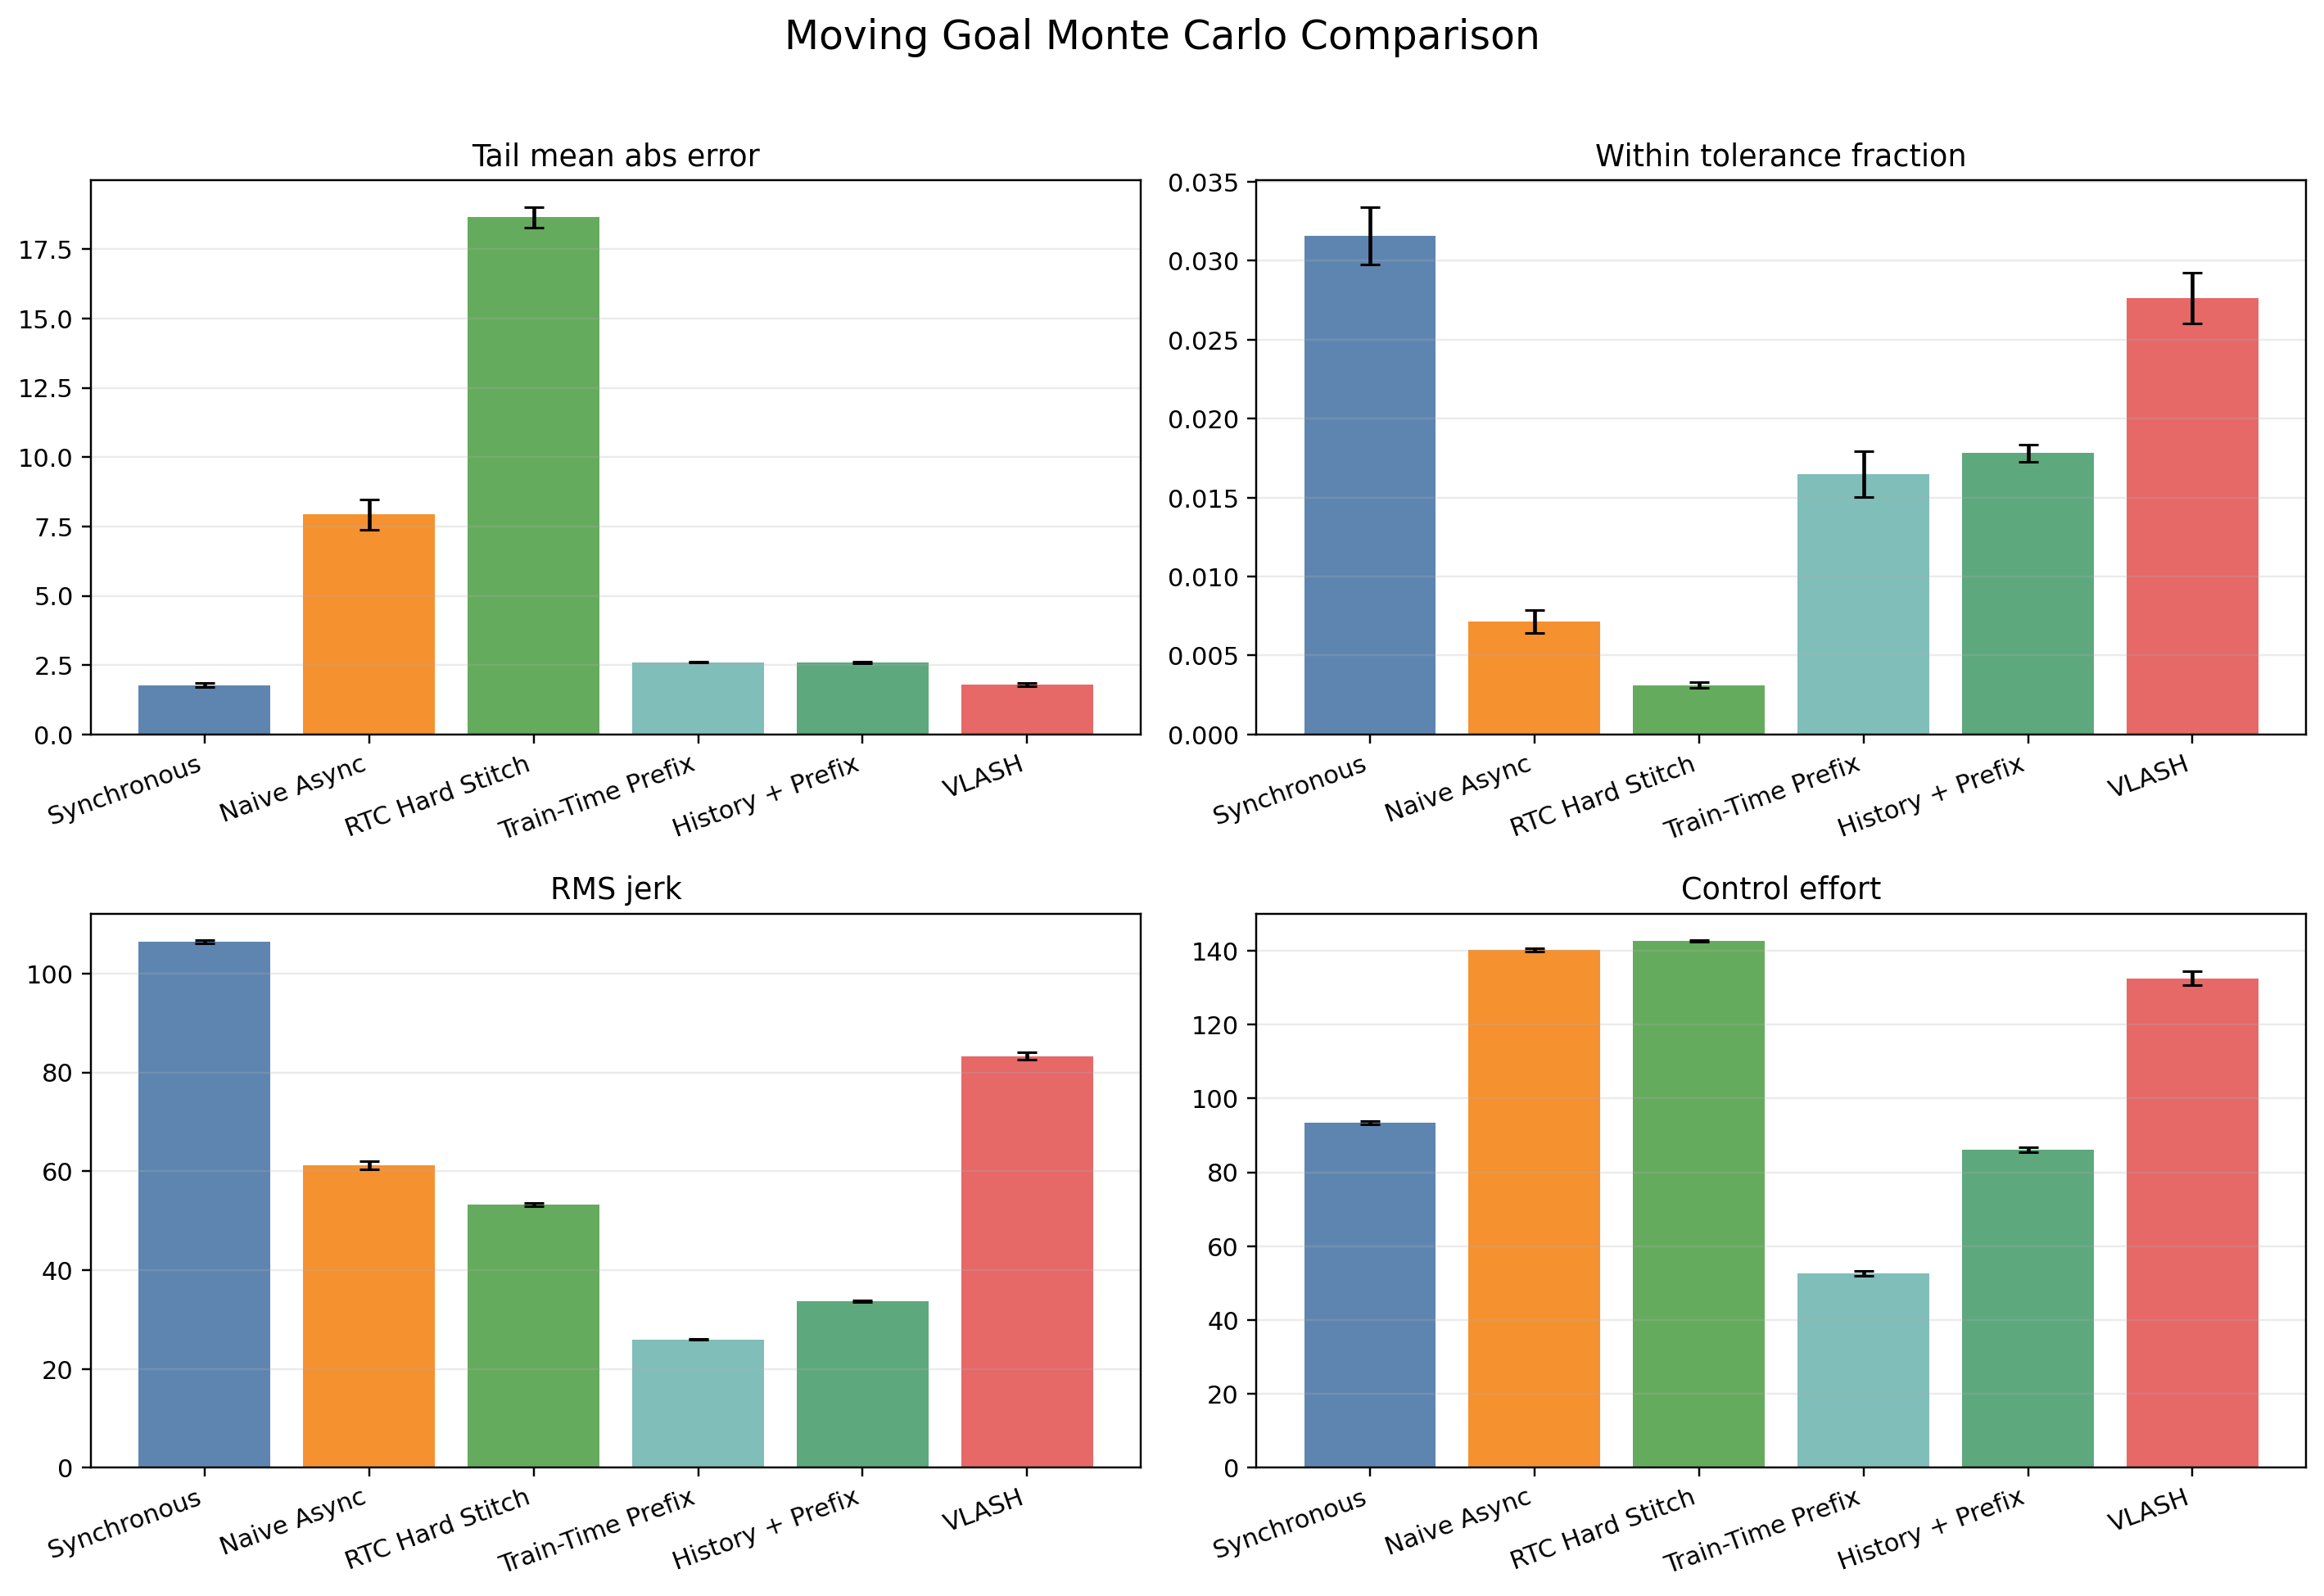
\includegraphics[width=\textwidth]{../outputs/async_chunking_dynamic_monte_carlo.png}
  \caption{Monte Carlo aggregates for the moving-goal setting.}
\end{figure}

\begin{table}[H]
\centering
\begin{tabular}{lrrrr}
\toprule
Method & Within tol. (\%) & Tail MAE & Final error & RMS jerk \\
\midrule
Synchronous & 3.2 & 1.781 & 1.617 & 106.4 \\
Naive Async & 0.7 & 7.925 & 8.059 & 61.2 \\
RTC Hard Stitch & 0.3 & 18.645 & 29.850 & 53.2 \\
Train-Time Prefix & 1.6 & 2.602 & 1.065 & 26.0 \\
History + Prefix & 1.8 & 2.589 & 1.596 & 33.7 \\
VLASH & 2.8 & 1.798 & 1.340 & 83.3 \\
VLASH + Reflex & 2.7 & 1.672 & 1.235 & 81.0 \\
\bottomrule
\end{tabular}
\caption{Moving-goal metrics exported by the current script. Tail MAE denotes tail mean absolute error.}
\end{table}

This scenario is more ambiguous. \texttt{Naive Async} and \texttt{RTC Hard Stitch} remain poor. \texttt{Train-Time Prefix} dramatically reduces jerk and control effort relative to the stronger planners, but it still lags the moving reference. \texttt{History + Prefix} offers a small improvement in tracking occupancy over prefix-only conditioning, but not enough to become a stronger overall baseline. \texttt{VLASH} and \texttt{VLASH + Reflex} stay competitive on tracking error, yet the current metrics do not justify a blanket claim of dominance over every baseline. The right reading is that future-state alignment remains promising, while the present moving-goal setup still needs better uncertainty-aware evaluation.

\section{Delay Sweep}

\begin{figure}[H]
  \centering
  \includegraphics[width=\textwidth]{../outputs/async_chunking_delay_sweep.png}
  \caption{Moving-goal delay sweep. The current plot is most useful as an intuition aid rather than a definitive benchmark summary.}
\end{figure}

The delay sweep reinforces three narrow conclusions:
\begin{itemize}[leftmargin=1.5em]
  \item small delays are more forgiving for all methods,
  \item naive async degrades quickly as delay grows,
  \item the hard-stitch negative control becomes unstable quickly, which supports the claim that continuity constraints need more than prefix freezing alone.
\end{itemize}

\section{What This Toy Does and Does Not Establish}

The current artifact does establish:
\begin{itemize}[leftmargin=1.5em]
  \item delayed chunked control can fail even in a simple system if planning is stale,
  \item train-time prefix conditioning can recover part of the lost continuity,
  \item future-state alignment is a strong design direction in this toy.
\end{itemize}

It does \emph{not} establish:
\begin{itemize}[leftmargin=1.5em]
  \item that VLASH is generally best for real VLA deployment,
  \item that RTC is weak relative to VLASH,
  \item that the present moving-goal result is robust enough for strong comparative claims,
  \item or that the current benchmark structure is broad enough to stand in for manipulation or embodied control.
\end{itemize}

\section{Next Critical Steps}

The two benchmark-audit subagents converged on the same main point: the highest-value next work is not another toy variant, but turning the current comparison into a credible benchmark.

\subsection{1. Fix the Baseline Set}

Before extending the narrative, the comparison needs stronger baselines:
\begin{enumerate}[leftmargin=1.5em]
  \item either add a faithful RTC-style baseline with actual inpainting-like continuity repair or remove RTC-comparison language,
  \item add a history/recurrent baseline with access to stale observations and committed prefix,
  \item add a classical latency-compensation controller such as MPC or Smith-predictor replanning,
  \item and report reflex variants consistently if reflex control remains part of the story.
\end{enumerate}

\subsection{2. Break the Oracle Assumption}

The current setup is too close to ``future-state oracle beats a student of the same oracle.'' To fix that:
\begin{enumerate}[leftmargin=1.5em]
  \item train on one distribution and evaluate on shifted delays, horizons, disturbance magnitudes, and goal dynamics,
  \item separate the teacher used for labels from the controller evaluated at test time,
  \item and inject model mismatch into future-state prediction so \texttt{VLASH} is not scored with exact nominal rollout only.
\end{enumerate}

\subsection{3. Upgrade the Timing Model}

Real async control does not have a perfectly deterministic compute delay. The benchmark should:
\begin{enumerate}[leftmargin=1.5em]
  \item sample inference latency from a distribution,
  \item include deadline misses and queueing effects,
  \item and define what happens when the next chunk is late.
\end{enumerate}

\subsection{4. Improve Reporting Quality}

The current report uses only means. The next pass should:
\begin{enumerate}[leftmargin=1.5em]
  \item export per-trial results,
  \item add confidence intervals or bootstrap intervals,
  \item use paired-seed comparisons,
  \item and report additional metrics such as overshoot, timeout rate, tracking lag, and safety-style violations.
\end{enumerate}

\subsection{5. Expand Scenario Coverage}

The task family is still too narrow. The next benchmark version should include:
\begin{enumerate}[leftmargin=1.5em]
  \item static setpoint, moving target, step changes, and adversarial disturbances,
  \item sweeps over both delay and horizon,
  \item and at least one higher-dimensional constrained system.
\end{enumerate}

\section{Current Conclusion}

The present artifact is a useful toy note for reasoning about delayed chunked control, but not yet a credible benchmark. The strongest next move is to tighten the claims, add non-strawman baselines, break the oracle coupling between planner and evaluator, and rerun the study with uncertainty-aware reporting.

\end{document}
